% !TeX encoding = windows-1251
\documentclass[a4paper,12pt,fleqn]{article}
\usepackage{newlistok}
\usepackage{tikz}

\УвеличитьВысоту{1.5cm}
\УвеличитьШирину{1.5cm}
\renewcommand{\spacer}{\vfil}

\Заголовок{Комбинаторика\т 2}
\НомерЛистка{6}
\ДатаЛистка{11.2012}

\begin{document}
\СоздатьЗаголовок

\опр
Обозначим через $C_n^k$ количество $k$-элементных подмножеств множества из $n$ элементов. Например, $C_4^2 = 6$, так как у множества $\{1, 2, 3, 4\}$ есть ровно 6 двухэлементных подмножеств:
\equ{
\{1, 2\},\, \{1, 3\},\, \{1, 4\},\, \{2, 3\},\, \{2, 4\},\, \{3, 4\}.
}
Иначе говоря, величина $C_n^k$ равна числу способов выбрать $k$ предметов из $n$.
\копр

\задача
Комбинаторными методами (не используя явную формулу) докажите, что\\
\пункт
$C_n^k=C_n^{n-k}$;
\пункт
$C_n^{k-1}+C_n^k=C_{n+1}^k$;
\пункт
$C_n^k C_{n-k}^{m-k}=C_m^k C_n^m$.
\кзадача

\задача
Найдите явную формулу для $C_n^k$.
\кзадача

\putthere{167mm}{-8mm}{%
    %
    % План города
    %
    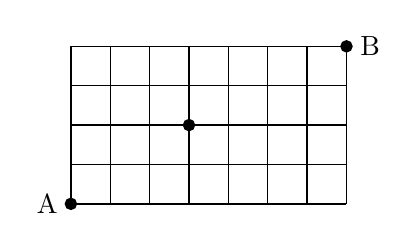
\begin{tikzpicture}[line width=.5pt]
        \draw[step=.5cm] (0,0) grid (3.5,2);
        \draw (-0.3,0) node {A};
        \draw (3.8,2) node {B};
        \filldraw [black] (0,0) circle (2pt)
                          (1.5,1) circle (2pt)
                          (3.5,2) circle (2pt);
    \end{tikzpicture}
}{7cm}{}
\vspace{-4mm}

\УстановитьГраницы{0cm}{5.3cm}
\задача
\пункт
На рисунке изображен план города
(линии\т это улицы, пересечения линий\т перекрестки).
На улицах введено одностороннее движение: можно
ехать только <<вверх>> или <<вправо>>. Сколько разных
маршрутов ведёт из точки $A$ в точку $B$?
\ВосстановитьГраницы
\пункт
Сколько из этих маршрутов не проходят через отмеченную на плане
точку внутри города?
\кзадача

\задача
Сколькими способами можно высадить в ряд 3 груши и 4 яблони?
\кзадача

\putthere{159mm}{-17mm}{%
    %
    % Треугольник Паскаля
    %
    $\begin{array}{ccccccccccc}
    &&&&& 1\\
    &&&& 1 && 1\\
    &&& 1 && 2 && 1\\
    && 1 && 3 && 3 && 1\\
    & 1 && 4 && 6 && 4 && 1\\
    .&.&.&.&.&.&.&.&.&.&.\\
    \end{array}$
}{7cm}{}
\vspace{-4mm}

\УстановитьГраницы{0cm}{65mm}
\опр
\emph{Треугольником Паскаля} называется треугольная таблица (см. рисунок справа), составленная из чисел согласно следующему правилу. По краям треугольника стоят единицы, а каждое из остальных чисел равно сумме двух, стоящих справа и слева над ним.
\копр

\задача
На рисунке выписаны первые 5 строк треугольника Паскаля. Напишите следующие 5 строк.
\кзадача
\ВосстановитьГраницы

\задача
Докажите, что $k$-ое число $n$-ой строки равно $C_n^k$
(строки нумеруются сверху вниз, начиная с нуля,
а числа в строках нумеруются слева направо, также начиная с нуля).
\кзадача

\задача
\label{diag1}
Возьмём любое число $C$ в треугольнике Паскаля и сложим все числа, начиная с него и идя по прямой направо-вверх. Докажите, что полученная сумма равна числу, стоящему под $C$ справа.
\кзадача


\задача
Выведите из задачи~\ref{diag1} формулы для сумм $1+\ldots+n$, $T_1+\ldots+T_n$, $\Pi_1+\ldots+\Pi_n$.
\кзадача

\сзадача
Как из предыдущей задачи вывести формулы для  $1^2+\ldots+k^2$, $1^3+\ldots+k^3$, \ldots?
\кзадача

\сзадача
В каких строках треугольника Паскаля все числа нечётные?
\кзадача

\сзадача
Найдите сумму $C_n^0 + C_{n-1}^1 + C_{n-2}^2 + \ldots$
\кзадача

\задача
Докажите, что при всех $n > 0$ выполнены неравенства $\dfrac{2^{2n}}{2n+1} \le C_{2n}^n \le 2^{2n-1}$.
\кзадача

\задача[Бином Ньютона]
Раскроем скобки и приведём подобные в выражении $(a+b)^n$. Возьмём любое слагаемое. Оно имеет вид $C\cdot a^k\cdot b^{n-k}$ (почему?). Докажите, что $C=C_n^k$.
\кзадача

\задача
Вычислите суммы:
\пункт
$C_n^0+C_n^1+C_n^2+\ldots+C_n^n$;
\пункт
$C_n^0-C_n^1+C_n^2-\ldots+(-1)^n C_n^n$;\\
\пункт[свёртка Вандермонда]
$C_p^0\cdot C_q^m+C_p^1\cdot C_q^{m-1}+\ldots+C_p^{m-1}\cdot C_q^1
+C_p^m\cdot C_q^0$;
\спункт
$(C_n^0)^2+(C_n^1)^2+\ldots+(C_n^n)^2$.
\кзадача

\задача
Сколько существует разбиений множества~$A$, состоящего из $n$~элементов,
\невСтрочку
\пункт
на три непересекающихся подмножества $A_1$, $A_2$, $A_3$, состоящих из~$k_1$, $k_2$ и~$k_3$ элементов соответственно, где~$k_1$, $k_2$, $k_3$\т такие заданные числа, что $k_1+k_2+k_3=n$;
\пункт
на $m$~непересекающихся подмножеств $A_1,\ldots, A_m$, состоящих из~$k_1,\ldots, k_m$ элементов соответственно, где $k_1,\ldots, k_m$\т такие заданные числа, что $k_1+\ldots+k_m=n$;
\пункт
на $m$ непересекающихся подмножеств $A_1,\ldots, A_m$ с~произвольным количеством элементов?
\кзадача





\ЛичныйКондуит{0mm}{6mm}
%\СделатьКондуит{6mm}{6mm}

%\GenXMLW

\end{document}




